\documentclass[11pt,a4paper]{article}
\usepackage[utf8x]{inputenc}

\usepackage[utf8x]{inputenc}

\usepackage{fancyhdr}

\usepackage[pdftex]{graphicx} % Required for including pictures
\usepackage[pdftex,linkcolor=black,pdfborder={0 0 0}]{hyperref} % Format links for pdf
\usepackage{calc} % To reset the counter in the document after title page
\usepackage{enumitem} % Includes lists

\usepackage[slovene]{babel}


\usepackage[normalem]{ulem}

\usepackage{textcomp}
\usepackage{eurosym}

\usepackage{xcolor}
\usepackage{graphicx}
\graphicspath{ {./images/} }

\usepackage{ amssymb } % extra math symbols
\usepackage{ amsmath } % extra math symbols
\usepackage{amsthm}
\usepackage{ dsfont } % font za množice
\usepackage{nicematrix}
% tabele
\usepackage{array}
\usepackage{wrapfig}
\usepackage{multirow}
\usepackage{tabularx}
\usepackage{multicol}
\usepackage{listings}
\usepackage{caption}
\usepackage{tikz,forest}
\usetikzlibrary{shapes, arrows.meta, arrows}
\usetikzlibrary{calc} % needed for BB

\newtheorem*{trditev}{Trditev}
\newtheorem*{izrek}{Izrek}
\newtheorem*{posledica}{Posledica}
\newtheorem*{definicija}{Definicija}

\frenchspacing % No double spacing between sentences
\setlength{\parindent}{0pt}
\setlength{\parskip}{0.5em}

\usepackage{mathtools}
\usepackage{blkarray, bigstrut} %
\usepackage{makecell}
\usepackage{nicematrix}

%\pagenumbering{gobble}

\lstset{basicstyle=\footnotesize\ttfamily, keywordstyle=\rmfamily\bfseries}

\DeclareCaptionLabelFormat{algocaption}{Algorithm \thenalg} % defines a new caption label as Algorithm x.y

\lstnewenvironment{algorithm}[1][] %defines the algorithm listing environment
{   
    %\refstepcounter{nalg} %increments algorithm number
    %\captionsetup{labelformat=algocaption,labelsep=colon} %defines the caption setup for: it ises label format as the declared caption label above and makes label and caption text to be separated by a ':'
    \lstset{ %this is the stype
        mathescape=true,
        %frame=tB,
        %numbers=left, 
        numberstyle=\tiny,
        basicstyle=\scriptsize, 
        keywordstyle=\color{black}\bfseries\em,
        keywords={,vhod, izhod, vrni, dokler, izvajaj, konec, zanke} %add the keywords you want, or load a language as Rubens explains in his comment above.
        %numbers=left,
        %xleftmargin=.04\textwidth,
        %#1 % this is to add specific settings to an usage of this environment (for instnce, the caption and referable label)
    }
}
{}
\usepackage{layouts}
\usepackage{floatrow}
\newfloatcommand{capbtabbox}{table}[][\FBwidth]

\definecolor{codegreen}{rgb}{0,0.6,0}
\definecolor{codegray}{rgb}{0.5,0.5,0.5}
\definecolor{codepurple}{rgb}{0.58,0,0.82}
\definecolor{backcolour}{rgb}{0.95,0.95,0.92}

\lstdefinestyle{mystyle}{
    basicstyle=\small,
    language=python, 
    breaklines, tabsize=2, 
    frame=leftline,xleftmargin=10pt,xrightmargin=10pt,framesep=10pt
}

\pagestyle{fancy}
\fancyhf{}
\rhead{Jernej Jezeršek}
\lhead{Matematika z računalnikom}
\rfoot{\thepage}

\begin{document}
\part*{Prepoznavanje zvokov cajona}
{\Large Končno poročilo}

\section{Problem}
Rad bi naredil sistem, ki posluša igranje cajona\footnote{\textbf{cajon} [kahón] - tolkalo v obliki lesene resonančne škatle, na kateri se sedi in udarja po sprednji stranici, navadno z roko, lahko z različnimi udarjalkami, v notranjosti ima lahko napeto žico, mrežico, z dodanimi kraguljčki, značilno za perujsko glasbo, v zadnjem času tudi za špansko glasbo, uporablja se ga tudi kot priročno alternativo klasičnim bobnarskim kompletom}, v realnem času prepoznava zvoke udarcev in glede na zaznave predvaja nove sintetične zvoke. Ta problem sem razdelil na dva dela:
\begin{enumerate}
    \item zaznava udarcev
    \item klasifikacija zvokov
\end{enumerate}
Prvi del sem že rešil z uporabo znanega algoritma za zaznavo udarcev (\emph{onset beat detection}). Drugemu delu pa se bom posvetil v tem projektu. Cajon lahko ustvari dva različna zvoka. Če igramo po spodnjem delu inštrumenta dobimo nižji zvok (kick), če pa igramo po zgornjem delu pa dobimo višji zvok (snare). Poleg tega se zvoki razlikujejo glede na moč udarca. 

Cilj tega projekta je razviti model, ki bo zvoke klasificiral v dva razreda (kick in snare). Ta problem postane težji, ko dodamo zahtevo, da mora model delovati v (skoraj) realnem času. To pomeni, da lahko za klasifikacijo uporabi le majhen del zvočnega signala (1 do 2 ms). Tako nizka zakasnitev je potrebna, da lahko med igranjem dodajamo druge zvoke ne da bi igralec opazil zakasnitev.


\section{Orodja}
Odločil sem se za uporabo programskega jezika Python, saj ima veliko zbirko knjižnic za obdelavo podatkov in strojno učenje. Za ta projekt sem uporabil oziroma nameravam uporabiti (med drugim) naslednje knjižnice: 
\begin{itemize}
    \item \texttt{scipy} - za branje in obdelavo zvočnih signalov
    \item \texttt{numpy} - za delo z večdimenzionalnimi seznami
    \item \texttt{scikit-learn} - za klasične metode strojnega učenja
    \item \texttt{tensorflow} - za delo z nevronskimi mrežami
    \item \texttt{matplotlib} - vizualizacija signalov in rezultatov
\end{itemize}

\section{Podatkovna množica}
Za testiranje različnih klasifikacijskih modelov je potrebna čim večja podatkovna množica. Za začetek sem ustvaril podatkovno množico iz zvokov svojega cajona. Za vsak razred (\emph{kick, snare}) in štiri različne jakosti (\emph{piano, mezzo piano, mezzo forte, forte}) sem posnel približno 60 zvokov (vse skupaj 264 zvokov `kick' in 277 zvokov `snare') in jih s pomočjo algoritma za zaznavo udarcev razdelil na posamezne vzorce. Ker je ta množica relativno majhna, sem pri nekaterih pristopih uporabil pristop bogatenja podatkov (data augmentation) in z dodajanjem šuma, spremembo jakosti, frekvence, hitrosti in zamika ustvaril nove vzorce.

Poleg tega sem posnel testno zvočno sled na kateri sem igral mešane udarce z različno jakostjo in v različnih ritmih. To zvočno sled bom uporabil za testiranje celotnega sistema.

Na sliki~\ref{fig:primer_kick_snare} je prikazan primer izluščenega zvočnega signala udarca `kick' in `snare'. Vidimo, da sta signala precej različna. Oba signala imata približno enako osnovno frekvenco okrog 50 Hz, vendar se razlikujeta v višjih frekvencah. Signal `snare' ima veliko bolj intenzivne in hitrejše oscilacije medtem, ko je `kick' zelo podoben sinusoidnemu signalu. To je dober znak, da bo tudi klasifikator lahko ločil med tema dvema razredoma.

\begin{figure}[h]
    \centering
    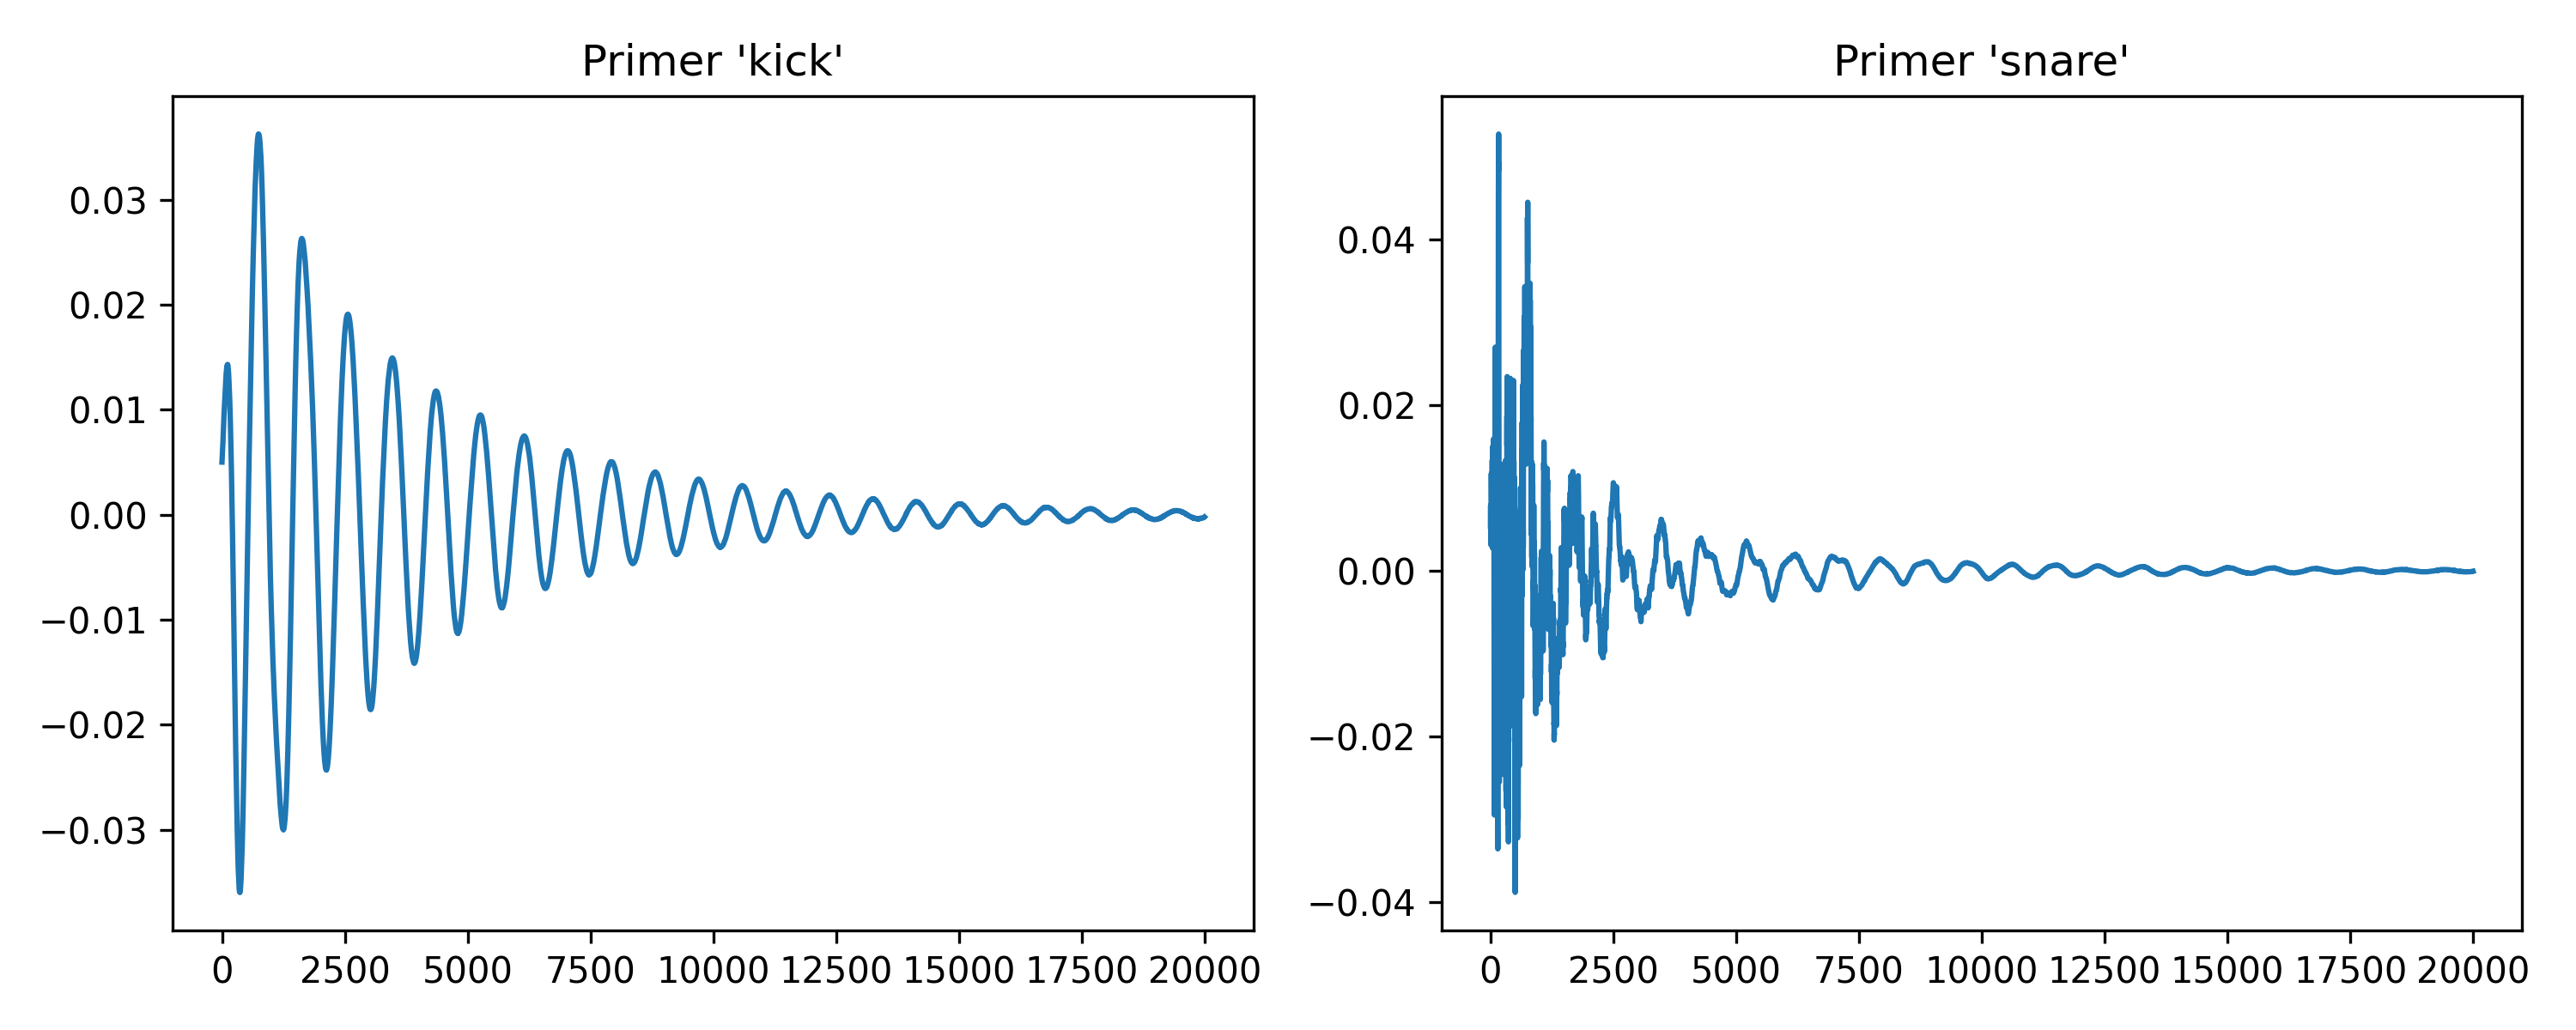
\includegraphics[width=\textwidth]{img/primer_kick_snare.png}
    \caption{Primer zvočnega signala udarca 'kick' in 'snare'.}
    \label{fig:primer_kick_snare}
\end{figure}

Vendar pa moramo pri gradnji klasifikacijskega algoritma upoštevati, da bo model imel na voljo le majhen del zvočnega signala (1 do 2 ms). Zaradi lažje implementacije Fourierove transofrmacije sem velikost okna omejil na potence števila 2. Na sliki~\ref{fig:primer_kick_snare_windows_hard} je prikazan primer zvočnega signala udarca `kick' in `snare' z označenimi velikostmi oken. Velikost okna je podana v številu vzorcev (\emph{sample rate}). V tem primeru so posnetki vzorčeni s frekvenco 44100 Hz, kar pomeni, da je 1 ms enak 44 vzorcem. Spodnja tabela prikazuje trajanje v milisekundah za različno število vzorcev. Seveda bi radi, da kalsifikacijski algoritem doseže čim višjo klasifikacijsko točnost z čim manjšim oknom.

\begin{center}
    \begin{tabular}{c c}
        \textbf{Število vzorcev} & \textbf{Trajanje (ms)} \\
        \hline
        64 & $\frac{64}{44100} \times 1000 \approx 1.45$ \\
        128 & $\frac{128}{44100} \times 1000 \approx 2.90$ \\
        256 & $\frac{256}{44100} \times 1000 \approx 5.80$ \\
        512 & $\frac{512}{44100} \times 1000 \approx 11.61$ \\
        \hline
    \end{tabular}
\end{center}

\begin{figure}[h]
    \centering
    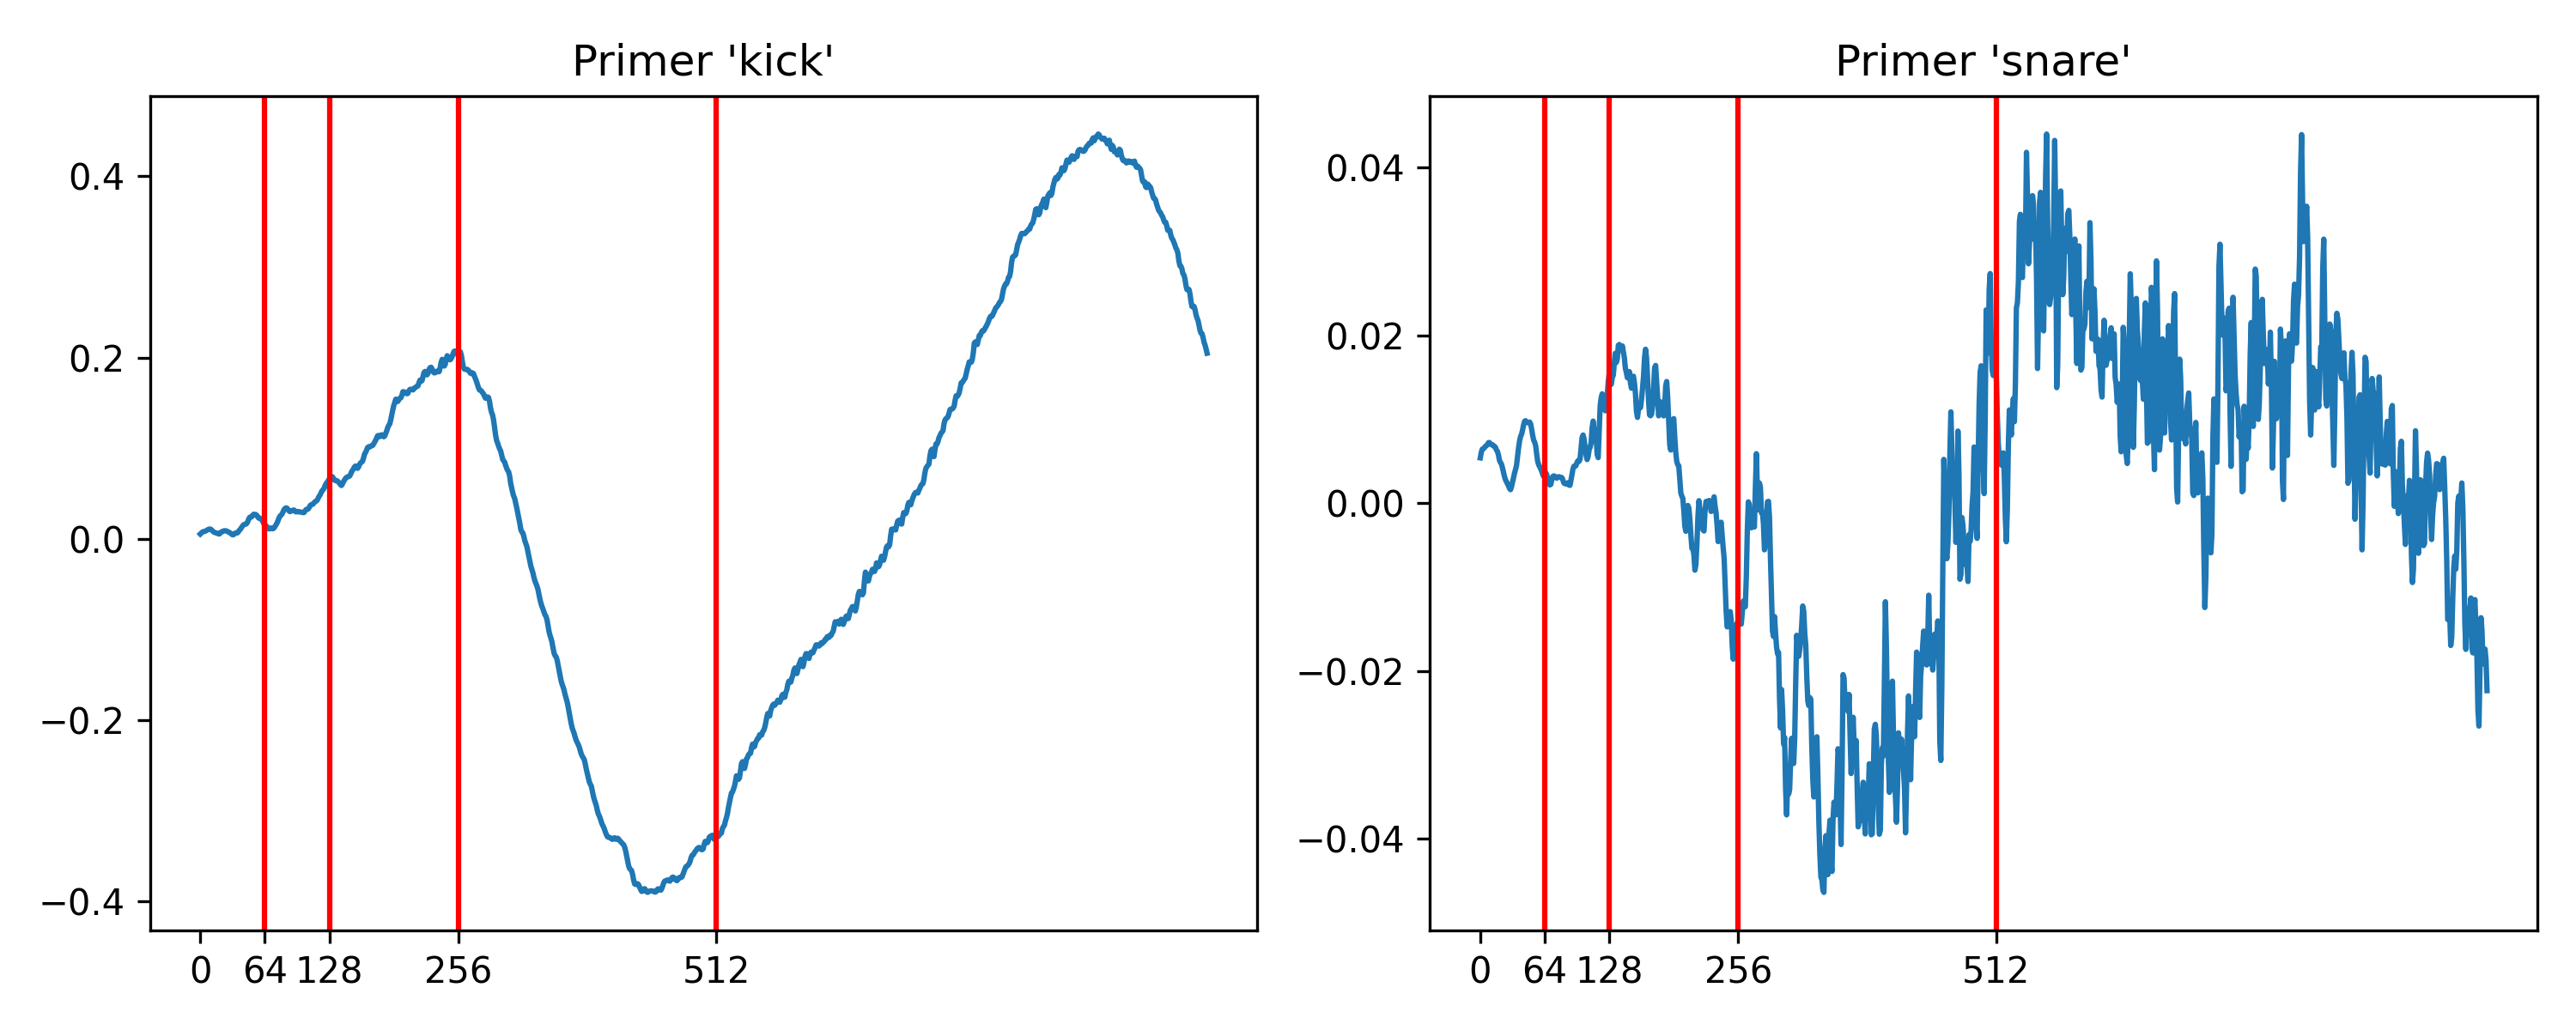
\includegraphics[width=\textwidth]{img/primer_kick_snare_windows_hard.png}
    \caption{Primer zvočnega signala udarca 'kick' in 'snare' z označenimi velikosti oken.}
    \label{fig:primer_kick_snare_windows_hard}
\end{figure}


Podatkovno množico sem razdelil na učno in testno množico tako, prva vsebuje 409 druga pa 132 zvokov. Vse modele sem učil le na učni množici, testiral pa na testni množici. 

\section{Testiranje modelov}
V nadaljevanju bom predstavil rezultate klasifikacije glede na uporabo različnih značilk, klasifikacijskih modelov in velikosti oken.

\subsection{Statistične značilke}
Izbral sem naslednje statistične značilke:
\begin{itemize}
    \item \textbf{min, max, povprečje, standardni odklon} - osnovne statistične značilke
    \item \textbf{kurtosis} - $\text{Kurt}(X) = E\left[ \left( \frac{X - \mu}{\sigma} \right)^4 \right] $
    \item \textbf{skewness} - $\text{Skew}(X) = E\left[ \left( \frac{X - \mu}{\sigma} \right)^3 \right] $
    \item \textbf{percentil} - izbral sem 25, 75, 90, 95 percentil
    \item \textbf{kvartilni razmik - IQR}
\end{itemize}

Značilke sem zložil v vektor in preizkusil različne klasifikacijske modele, ki jih ponuja knjižnica \texttt{scikit-learn}. In sicer:
\begin{itemize}
    \item \textbf{k najbljižjih sosedov - kNN} s $k=2$, saj imamo dva razreda  
    \item \textbf{model podpornih vektorjev - SVC} s skaliranjem značilk. Najboljše rezultate sem dobil z uporabo skaliranja značilk in regularizaciskim parametrom $C=1$.
    \item \textbf{logistična regresija} z L2 normo in reqularizacijskim parametrom $C=1$
    \item \textbf{naključni gozd} z maksimalno globino 20 in 100 drevesi.
    \item \textbf{gosta nevronska mreža} kjer je vhodna plast dovisna od velikosti okna dve notranji plasti pa sta veliki 16 in 4 nevrone.
\end{itemize}

Rezultati za posamezne modele in velikosti oken so prikazani v tabelah spodaj. Za vsak model sem izračunal točnost na testni množici (\emph{točnost}), točnost na učni množici (\emph{učna točnost}), čas učenja in čas napovedi za celo testno množico.

\begin{center}
\begin{tabular}{r | c c c c c}
    \multicolumn{5}{c}{k najbližjih sosedov}\\
    \tiny{Velikost okna} & \small{64} & \small{128} & \small{256} & \small{512}\\ \hline
    \tiny{Točnost} & \small{0.73} & \small{0.80} & \small{0.86} & \small{0.98}\\
    \tiny{Učna točnost} & \small{0.85} & \small{0.87} & \small{0.94} & \small{0.99}\\
    \tiny{Čas učenja [ms]} & \small{1.00} & \small{1.00} & \small{1.00} & \small{1.00}\\
    \tiny{Čas napovedi [ms]} & \small{1.70} & \small{2.00} & \small{2.01} & \small{2.00}\\
    \end{tabular}

\begin{tabular}{r | c c c c c}
    \multicolumn{5}{c}{SVC z normalizacijo}\\
    \tiny{Velikost okna} & \small{64} & \small{128} & \small{256} & \small{512}\\ \hline
    \tiny{Točnost} & \small{0.87} & \small{0.94} & \small{0.95} & \small{0.96}\\
    \tiny{Učna točnost} & \small{0.82} & \small{0.91} & \small{0.96} & \small{0.98}\\
    \tiny{Čas učenja [ms]} & \small{3.86} & \small{2.02} & \small{1.50} & \small{2.00}\\
    \tiny{Čas napovedi [ms]} & \small{1.00} & \small{0.00} & \small{0.00} & \small{0.00}\\
    \end{tabular}

\begin{tabular}{r | c c c c c}
    \multicolumn{5}{c}{Logistična regresija}\\
    \tiny{Velikost okna} & \small{64} & \small{128} & \small{256} & \small{512}\\ \hline
    \tiny{Točnost} & \small{0.80} & \small{0.72} & \small{0.63} & \small{0.88}\\
    \tiny{Učna točnost} & \small{0.76} & \small{0.75} & \small{0.67} & \small{0.86}\\
    \tiny{Čas učenja [ms]} & \small{2.00} & \small{2.27} & \small{2.01} & \small{2.00}\\
    \tiny{Čas napovedi [ms]} & \small{0.00} & \small{0.00} & \small{1.00} & \small{0.00}\\
    \end{tabular}

\begin{tabular}{r | c c c c c}
    \multicolumn{5}{c}{Naključni gozd}\\
    \tiny{Velikost okna} & \small{64} & \small{128} & \small{256} & \small{512}\\ \hline
    \tiny{Točnost} & \small{0.85} & \small{0.92} & \small{0.97} & \small{0.98}\\
    \tiny{Učna točnost} & \small{1.00} & \small{1.00} & \small{1.00} & \small{1.00}\\
    \tiny{Čas učenja [ms]} & \small{99.86} & \small{92.01} & \small{82.54} & \small{88.96}\\
    \tiny{Čas napovedi [ms]} & \small{2.00} & \small{2.00} & \small{2.51} & \small{2.00}\\
    \end{tabular}

\begin{tabular}{r | c c c c c}
    \multicolumn{5}{c}{Gosta nevronska mreža (32, 4)}\\
    \tiny{Velikost okna} & \small{64} & \small{128} & \small{256} & \small{512}\\ \hline
    \tiny{Točnost} & \small{0.79} & \small{0.86} & \small{0.95} & \small{0.99}\\
    \tiny{Učna točnost} & \small{0.77} & \small{0.84} & \small{0.97} & \small{1.00}\\
    \tiny{Čas učenja [ms]} & \small{428.72} & \small{246.72} & \small{281.31} & \small{326.81}\\
    \tiny{Čas napovedi [ms]} & \small{0.00} & \small{0.00} & \small{0.00} & \small{0.00}\\
    \end{tabular}
\end{center}

Za najboljši model se je izkazal SVC, saj je dosegel najvišjo točnost za najmanjši velikosti okna 64 in 128. Za večje velikosti oken pa sta bila najboljša modela naključni gozd in gosta nevronska mreža. Kljub temu mislim, da je SVC najboljši model saj ima tudi najnižji čas napovedi in učenja.



\subsection{Spektralne značilke}
Ker se zvoki `kick' in `snare' razlikujejo v višjih frekvencah, bi lahko spektralne značilke bile dober indikator za razlikovanje med tema dvema razredoma. Slika~\ref{fig:primer_kick_snare_fft128} prikazuje primer izseka zvočnega signala udarca `kick' in `snare' in pripadajočo Fourierovo transformacijo. Na levi strani so prikazane jakosti nizkih frekvenc na desni pa visokih. 

\begin{figure}[h]
    \centering
    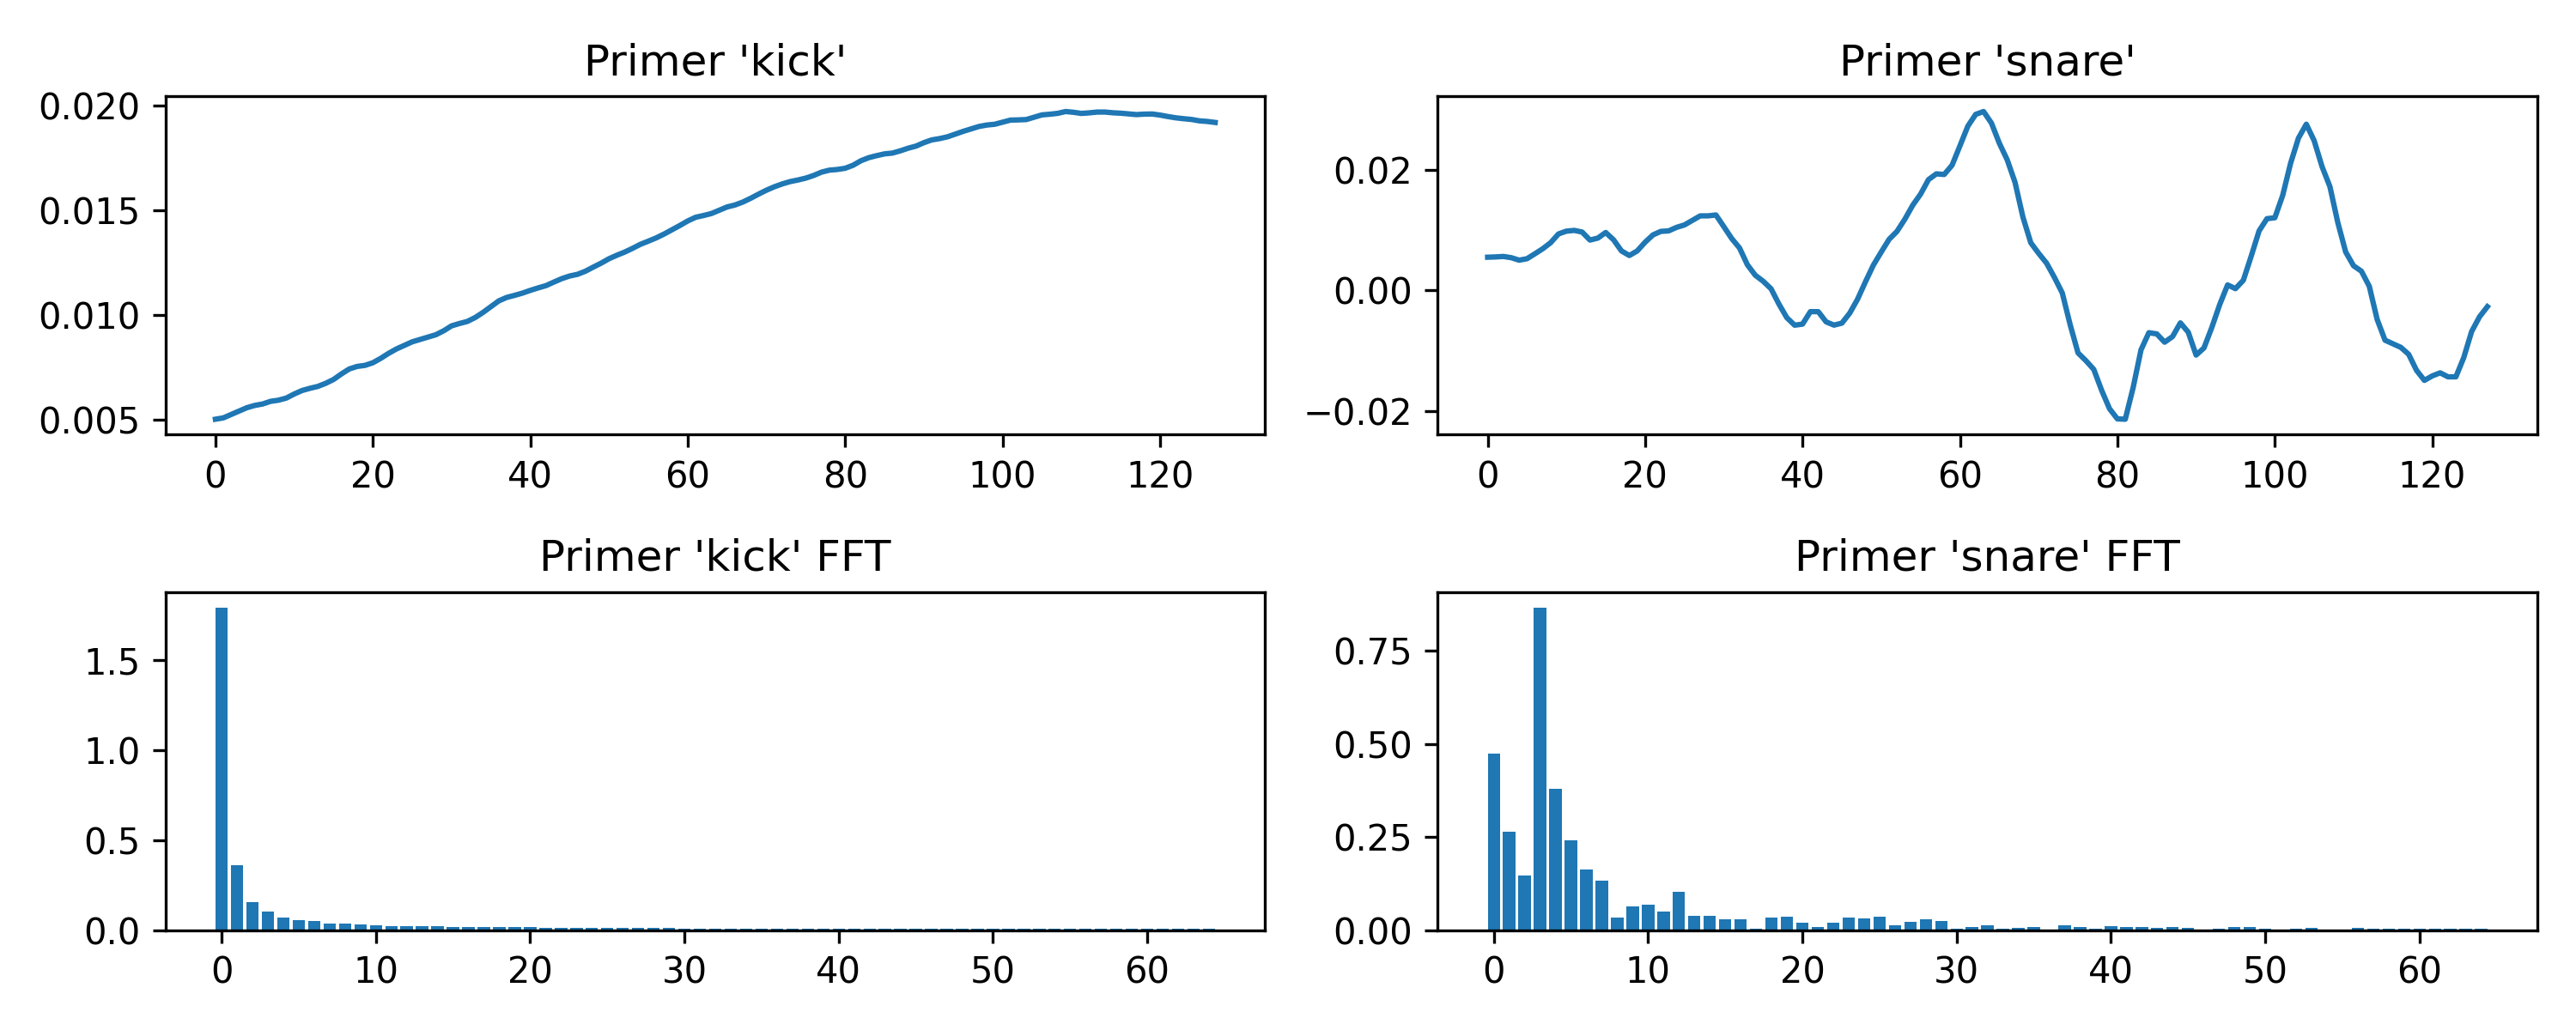
\includegraphics[width=\textwidth]{img/primer_kick_snare_fft128.png}
    \caption{Primer izseka (velikost okna 128) signala udarca 'kick' in 'snare' in pripidajoča Fourierova transformacija.}
    \label{fig:primer_kick_snare_fft128}
\end{figure}

Da bi preveril kako dobro se da ločiti zvoke samo iz vektorja jakosti po frekvencah, sem uporabil metodo glavnih komponent (PCA) za zmanjšanje dimenzionalnosti. Na sliki~\ref{fig:pca_fft} so prikazane projekcije vektorja frekvenc vzorcev v nižje dimenzionalen prostor. Vidimo, da večje kot je okno, bolj se razredi ločijo.

\begin{figure}[h]
    \centering
    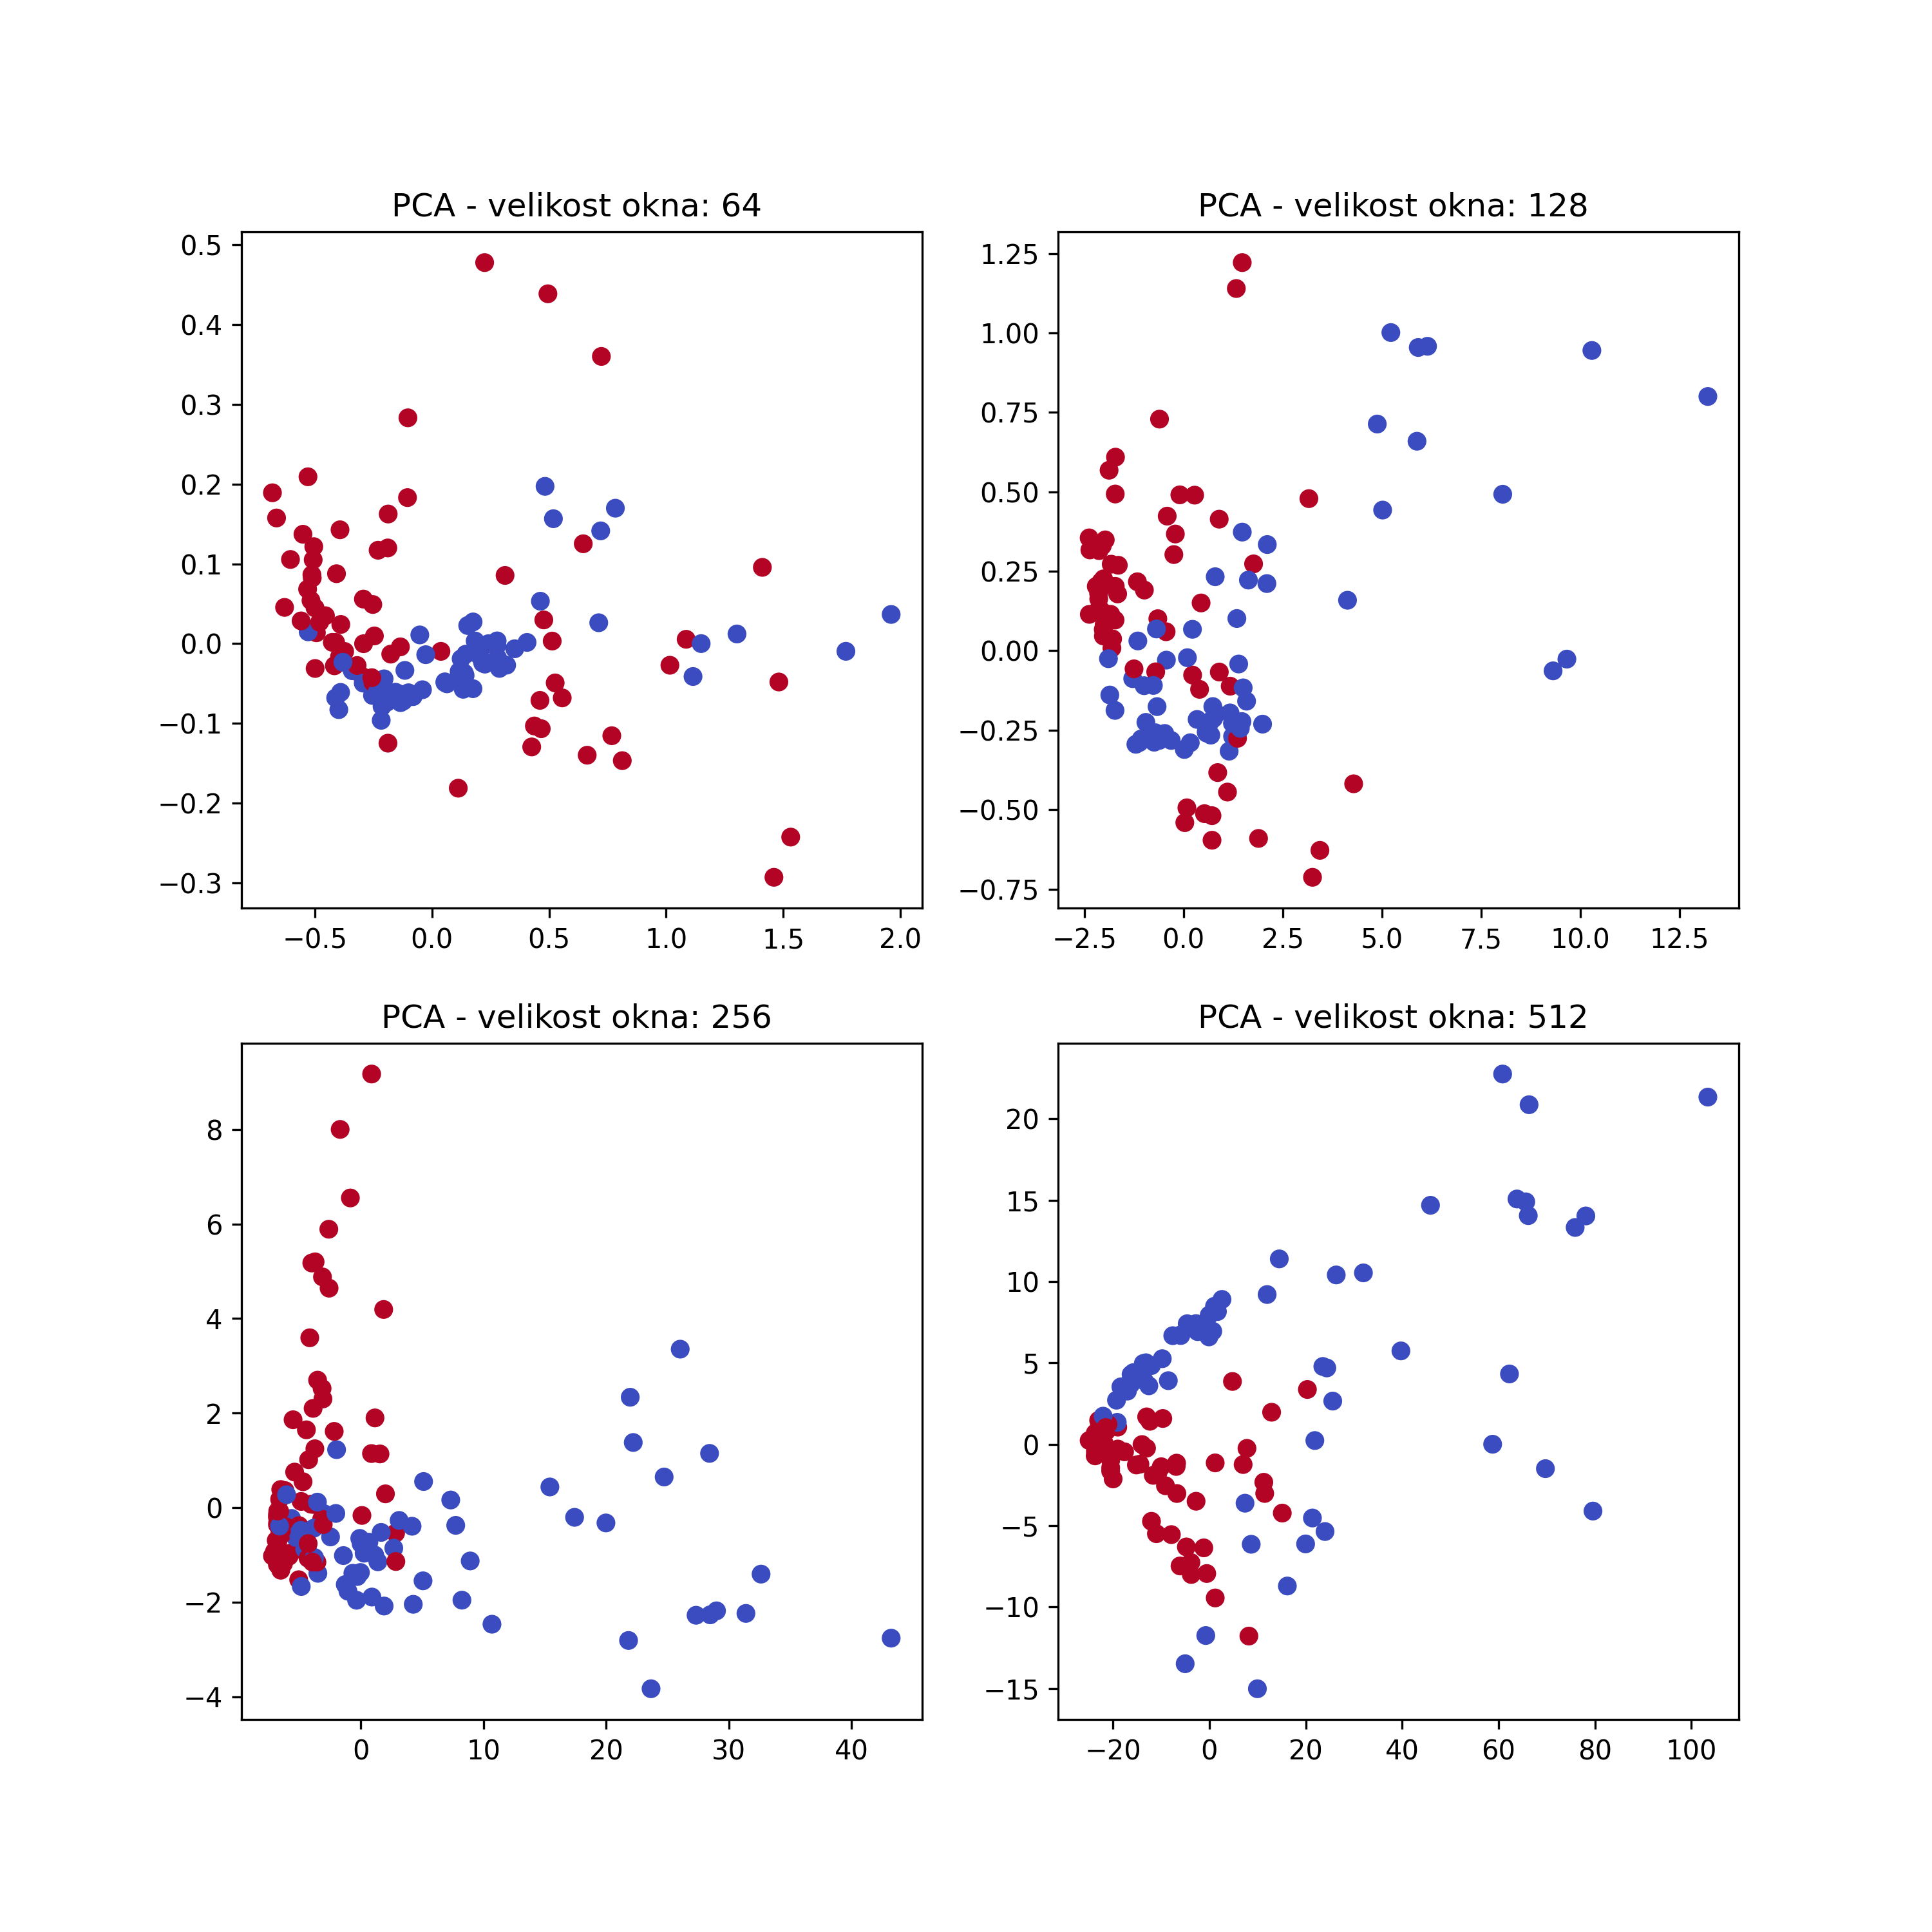
\includegraphics[width=\textwidth]{img/pca_fft.png}
    \caption{Prikaz testnih vzorcev v prostoru prvih dveh glavnih komponent za različne velikosti oken.}
    \label{fig:pca_fft}
\end{figure}

Nato sem preiskusil različne različne klasifikacijske modele, ki jih ponuje knjižnica \texttt{scikit-learn}. In sicer
\begin{itemize}
    \item \textbf{k najbljižjih sosedov - kNN}  s $k=2$, saj imamo dva razreda  
    \item \textbf{model podpornih vektorjev - SVC}  s skaliranjem značilk. Najboljše rezultate sem dobil z uporabo skaliranja značilk in regularizaciskim parametrom $C=0.7$.
    \item \textbf{logistična regresija}  z L2 normo in reqularizacijskim parametrom $C=1$
    \item \textbf{naključni gozd}  z maksimalno globino 20 in 100 drevesi.
    \item \textbf{gosta nevronska mreža}  kjer je vhodna plast dovisna od velikosti okna dve notranji plasti pa sta veliki 128 in 16 nevronov.
\end{itemize}

Rezultati za posamezne modele in velikosti oken so prikazani v tabelah spodaj. 

\begin{center}

    \begin{tabular}{r | c c c c c}
        \multicolumn{5}{c}{k najbližjih sosedov}\\
        \tiny{Velikost okna} & \small{64} & \small{128} & \small{256} & \small{512}\\ \hline
        \tiny{Točnost} & \small{0.81} & \small{0.82} & \small{0.94} & \small{0.97}\\
        \tiny{Učna točnost} & \small{0.86} & \small{0.89} & \small{0.97} & \small{0.96}\\
        \tiny{Čas učenja [ms]} & \small{0.51} & \small{0.00} & \small{0.42} & \small{0.00}\\
        \tiny{Čas napovedi [ms]} & \small{6.11} & \small{4.00} & \small{3.55} & \small{4.00}\\
        \end{tabular}

    \begin{tabular}{r | c c c c c}
        \multicolumn{5}{c}{SVC z normalizacijo}\\
        \tiny{Velikost okna} & \small{64} & \small{128} & \small{256} & \small{512}\\ \hline
        \tiny{Točnost} & \small{0.86} & \small{0.92} & \small{0.98} & \small{1.00}\\
        \tiny{Učna točnost} & \small{0.89} & \small{0.99} & \small{1.00} & \small{1.00}\\
        \tiny{Čas učenja [ms]} & \small{4.11} & \small{2.00} & \small{1.11} & \small{2.00}\\
        \tiny{Čas napovedi [ms]} & \small{0.50} & \small{0.00} & \small{0.00} & \small{0.00}\\
        \end{tabular}

    \begin{tabular}{r | c c c c c}
        \multicolumn{5}{c}{Logistična regresija}\\
        \tiny{Velikost okna} & \small{64} & \small{128} & \small{256} & \small{512}\\ \hline
        \tiny{Točnost} & \small{0.79} & \small{0.78} & \small{0.96} & \small{0.94}\\
        \tiny{Učna točnost} & \small{0.78} & \small{0.85} & \small{0.96} & \small{1.00}\\
        \tiny{Čas učenja [ms]} & \small{8.23} & \small{16.57} & \small{16.54} & \small{45.93}\\
        \tiny{Čas napovedi [ms]} & \small{0.00} & \small{0.00} & \small{0.00} & \small{0.00}\\
        \end{tabular}

    \begin{tabular}{r | c c c c c}
        \multicolumn{5}{c}{Naključni gozd}\\
        \tiny{Velikost okna} & \small{64} & \small{128} & \small{256} & \small{512}\\ \hline
        \tiny{Točnost} & \small{0.86} & \small{0.95} & \small{0.97} & \small{0.97}\\
        \tiny{Učna točnost} & \small{1.00} & \small{1.00} & \small{1.00} & \small{1.00}\\
        \tiny{Čas učenja [ms]} & \small{153.31} & \small{187.75} & \small{261.79} & \small{275.57}\\
        \tiny{Čas napovedi [ms]} & \small{2.00} & \small{2.50} & \small{2.51} & \small{2.00}\\
        \end{tabular}

    \begin{tabular}{r | c c c c c}
        \multicolumn{5}{c}{Gosta nevronska mreža (128, 16)}\\
        \tiny{Velikost okna} & \small{64} & \small{128} & \small{256} & \small{512}\\ \hline
        \tiny{Točnost} & \small{0.86} & \small{0.95} & \small{0.98} & \small{0.99}\\
        \tiny{Učna točnost} & \small{0.88} & \small{0.98} & \small{1.00} & \small{1.00}\\
        \tiny{Čas učenja [ms]} & \small{470.75} & \small{586.31} & \small{882.55} & \small{581.52}\\
        \tiny{Čas napovedi [ms]} & \small{0.00} & \small{0.00} & \small{0.00} & \small{0.00}\\
        \end{tabular}
\end{center}


Za najboljši model se je spet izkazal model podpornih vektorjev, saj je dosegel najvičjo točnost za velikost okna 64, 256 in 512. Za velikost okna 128 pa je bil najboljši model naključni gozd. 


\subsection{Surov signal}

Za konec sem preizkusil še model s konvolucijsko nevronsko mrežo, ki deluje na surovem signalu. S tem modelom sem dosegel najboljšo klasifikacijsko točnost, je pa tudi najbolj računsko zahteven - za učenje potrebuje 22 s, kar je na pram ostalim modelom precej več. Poleg tega zahteva veliko večjo učno množico, da doseže robustno učenje. Zato sem podatkovno množico razširil z augmentiranjem podatkov na naslednje načine:
\begin{itemize}
    \item dodajanje šuma
    \item premikanje signala
    \item spreminjanje amplitude
    \item pohitritev in upočasnitev signala
\end{itemize}

Najbolj učinkovita metoda augmentiranja je bila zamikanje signala. Predvidevam, da je to zato ker se signali precej periodično ponavljajo in z zamikanjem dobimo nove podatke, ki pa so podobni originalnim. Poleg tega zamikanje lahko izboljša robustnost modela, saj bo na ta nači model bolje propoznal zvoke pri katerih se je detektor udarcel morda sprožil prepozno.

Za implementacijo konvolucijske nevronske mreže sem uporabil knjižnico \texttt{keras} in \texttt{tensorflow}. Model sem zgradil z naslednjimi sloji:
\begin{itemize}
    \item Vhodna plast (enake velikosti kot okno)
    \item Konvolucijska plst (4 filtri velikosti 3, pomik 1)
    \item Plast za združevanje (max pooling) (velikost 2)
    \item Gosta plast (32 nevronov)
    \item Gosta plast (16 nevronov)
    \item Končna gosta plst (1 nevron)
\end{itemize}

Spodnja tabela prikazuje rezultate modela za različne velikosti oken.

\begin{center}

    \begin{tabular}{r | c c c c c}
        \multicolumn{5}{c}{Konvolucijska nevronska mreža}\\
        \tiny{Velikost okna} & \small{64} & \small{128} & \small{256} & \small{512}\\ \hline
        \tiny{Točnost} & \small{0.97} & \small{0.99} & \small{0.99} & \small{0.99}\\
        \tiny{Učna točnost} & \small{0.97} & \small{0.99} & \small{0.99} & \small{0.99}\\
        \tiny{Čas učenja [s]} & \small{22} & \small{33} & \small{39} & \small{56}\\
        \tiny{Čas napovedi [ms]} & \small{0.5} & \small{0.5} & \small{0.6} & \small{0.6}\\
        \end{tabular}

\end{center}

\section{Implementacija na mikrokrmilniku}
Celoten sistem sem implementiral na mikrokrmilniku ESP32-S3. Mikrokrmilnik je povezan z modulom za zajem zvoka, ki pretvori analogni signal v digitalnega in ga prek protokola I2S pošlje mikrokrmilniku (slika~\ref{fig:vezje}). Mikrokrmilnik prepoznava udarce in glede na zaznave predvaja v naprej določene zvoke.

\begin{figure}[h]
    \centering
    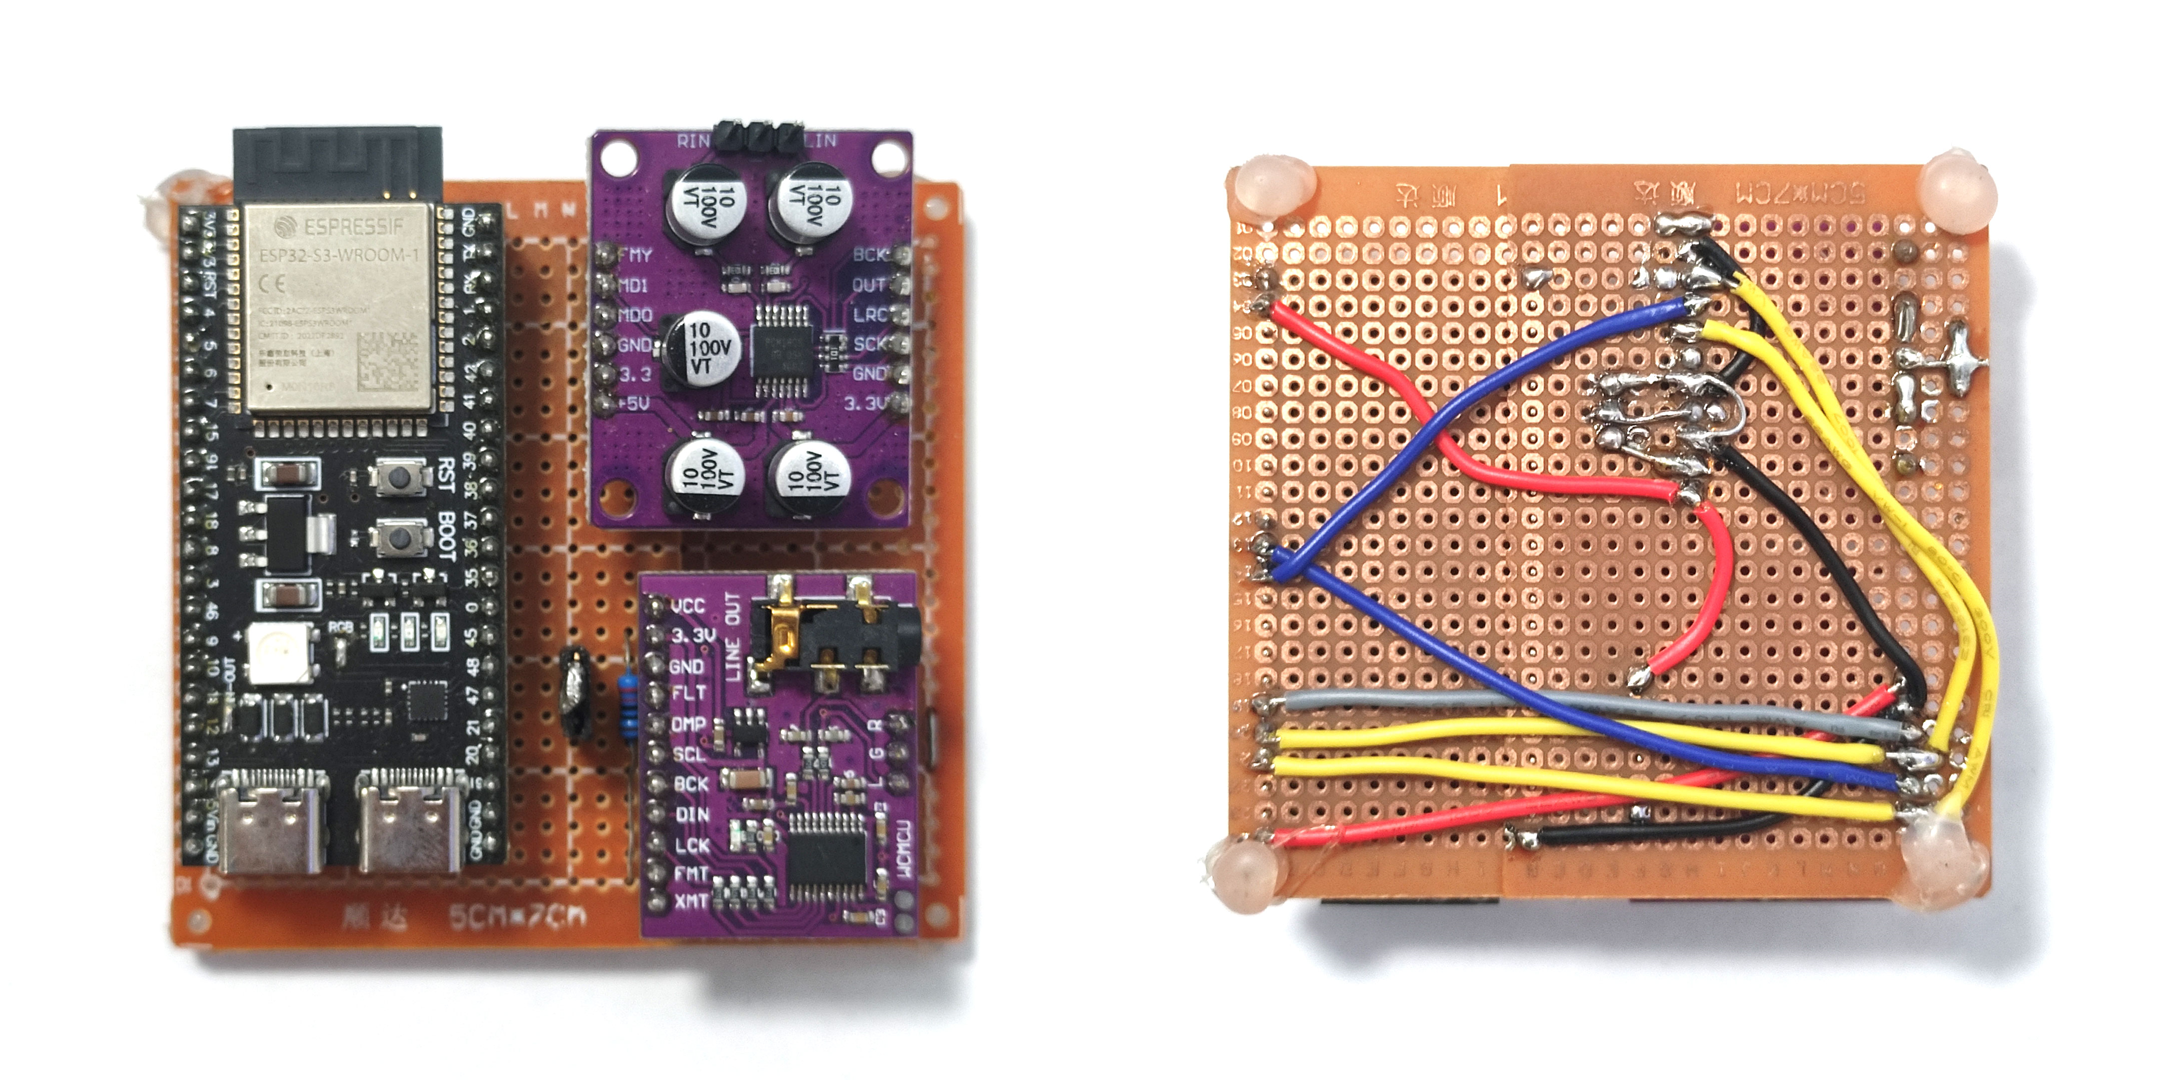
\includegraphics[width=\textwidth]{img/vezje.png}
    \caption{Mikrokrmilnik ESP32-S3 povezan z ADC in DAC moduloma.}
    \label{fig:vezje}
\end{figure}

Za programiranje mikrokrmilmika sem uporabil ogrodje ESP-IDF, ki omo\-go\-ča deljenje programa na več procesov in paralelno izvajanje. Na mikrokrmilniku sem implementiral model konvolucijske nevronske mreže, ki sem ga prej naučil na računalniku. Za poganjanje modela na mikrokrmilniku sem uporabil knjižnico \texttt{tensorflow-lite}.


\section*{Zaključek}

Ugotovil sem, da je najbolj točen model za klasifikacijo zvokov cajona konvolucijska nevronska mreža. Model je dovolj majhen, da ga lahko uporabljamo na mikrokrmilniku ESP32-S3. V prihodnosti bi rad klasifikator še izboljšal z uporabo večjih podatkovnih množic in morda z uporabo večjih modelov. Poleg tega bi rad preiskusi, če bi lahko podoben sistem uporabil za klasifikacijo večjega števila zvokov. Naprimer da bi lahko zaznal še udarce po straneh cajona.


\end{document}